\documentclass[11pt,a4paper]{article}

\usepackage[utf8]{inputenc}
\usepackage[margin=2.5cm]{geometry}
\usepackage{amsmath,amssymb,amsthm}
\usepackage{booktabs,tabularx,array}
\usepackage{enumitem}
\usepackage{tikz}
\usetikzlibrary{arrows.meta,positioning,patterns}
\usepackage[hidelinks]{hyperref}
\usepackage{xurl}

\newtheorem{proposition}{Proposition}
\newtheorem{lemma}[proposition]{Lemma}
\newtheorem{corollary}[proposition]{Corollary}
\theoremstyle{remark}
\newtheorem{remark}[proposition]{Remark}
\newcommand{\code}[1]{\path{#1}}
\urlstyle{tt}
\newcolumntype{Y}{>{\raggedright\arraybackslash}X}
\newcommand{\sgn}{\operatorname{sign}}
\setlength{\emergencystretch}{3em}
\hyphenation{ex-po-nen-ti-a-tion}

\title{CE114: rational $d$ for $36n^3-19=-2d\,x^2\bigl(-(x+6n)+\sqrt{\cdots}\,\bigr)$\\
via the Booker--Sutherland gap search\\[2pt]
\large rationale and modus operandi of the current scripts}
\author{Jamal Agbanwa}
\date{12 November 2026; revised 13 November 2026}

\begin{document}
\maketitle

\begin{abstract}
The scripts in \texttt{114 /Algorithm for computation /gap-search/} look for rational values of
$d$ for which the equation
$36n^3-19=-2d\,x^2\bigl(-(x+6n)+\sqrt{(x+6n)^2+(36n^3-19)/x}\bigr)$ has a point with an
integral square root (integer chart) or with $x=X/2$ and square root $Y/2$, $X,Y$ odd (half
chart). Both acceptable results are exactly the integer solutions of $a^3+b^3+c^3=114$: every
solution gives one rational $d$ of the first kind and two of the second.

Following Dr.\ Grechuk's advice to use the best available algorithm and to aim it beyond the
range already checked, the production computation is the Booker--Sutherland method. It is
restricted to the part of the search space that their 2020 search for $k=114$ left out:
$\delta=|a+b|>10^{19}/54$, with $3.847\,\delta\le|c|\le64\,\delta$. A converter then turns
any solution found into its three values of $d$, verified on the original equation. The
campaign is sized for 1{,}800 core-hours.

This note gives the reduction with proofs, what is already excluded, the heuristic that
selects the region, the algorithm step by step, the operating procedure, the validation and
review evidence, the status of the folder's earlier programs, and the limits of the method.
Under the Booker--Sutherland heuristic, the run has about a $1$ in $145{,}000$--$165{,}000$
chance of producing a solution. (It was $1$ in $190{,}000$--$200{,}000$ before the 2-adic rule
of Proposition~\ref{prop:twoadic} and the mod-24 wheel, which together make the engine
about $1.3$ times faster.)
\end{abstract}

\tableofcontents

%====================================================================
\section{Purpose and target}

Let
\begin{equation}\label{eq:E}\tag{E}
  36n^3-19=-2d\,x^2\bigl(-(x+6n)+s\bigr),\qquad
  s=\sqrt{(x+6n)^2+\frac{36n^3-19}{x}}\ \ge 0 .
\end{equation}
The task is to find rational $d$ for which \eqref{eq:E} has a point of one of the following
kinds:
\begin{enumerate}[label=\textbf{Result \arabic*.},leftmargin=*]
  \item \emph{Integer chart:} $n,x\in\mathbb Z$ and $s\in\mathbb Z$.
  \item \emph{Half chart:} $n\in\mathbb Z$, $x=X/2$ and $s=Y/2$ with $X,Y$ odd integers.
\end{enumerate}
The code lives in
\url{https://github.com/JAgbanwa/SomethingNew/tree/main/114%20/Algorithm%20for%20computation%20/gap-search}.
This note describes the revision of 6 November 2026 (commits \texttt{d19a6a3} and
\texttt{194e6ca}). The revision of 13 November 2026 adds Remark~\ref{rem:delta} (this $d$ is
not Booker--Sutherland's $\delta$), Proposition~\ref{prop:only} (Results~1 and~2 are the only
targets, and the only half-integral points that are representations of $114$), the new
cross-check \code{rational-d-search/} (Section~\ref{sec:older}), and the local conditions
$n\equiv0\pmod3$, $x\equiv7\pmod{12}$ of Result~1 (Proposition~\ref{prop:local}). The
$2$-adic part of the latter gives a new rule, Proposition~\ref{prop:twoadic}. The engine now
skips three quarters of the even $\delta$ before any root finding, which is about $1.26$
times faster on the same host. A mod-$24$ wheel in the sieve then stops the sieve from
visiting skipped $\delta$ at all, for about $3\%$ more (Section~\ref{sec:engine}). The search
is still $k=114$ only, and the region is unchanged.

%====================================================================
\section{The problem is exactly \texorpdfstring{$114=a^3+b^3+c^3$}{114 = a3 + b3 + c3}}\label{sec:reduction}

Throughout, write $N(n)=36n^3-19$ and $U=x+6n$, and more generally $36n^3-m$ with $k=6m$.
Production uses $m=19$, $k=114$.

\begin{proposition}[the cube identity]\label{prop:identity}
For $x\ne0$ put $A=-x+s$, $B=-x-s$, $C=2x+6n$, where $s$ is any number. Then
\[
  A^3+B^3+C^3-6m \;=\; -6x\Bigl(s^2-(x+6n)^2-\frac{36n^3-m}{x}\Bigr).
\]
\end{proposition}
\begin{proof}
$A^3+B^3=(A+B)\bigl((A+B)^2-3AB\bigr)=-2x(4x^2-3x^2+3s^2)=-2x^3-6xs^2$.
Also $C^3=8x^3+72x^2n+216xn^2+216n^3$. Adding,
\[
A^3+B^3+C^3-6m=6x^3+72x^2n+216xn^2+216n^3-6m-6xs^2 .
\]
The right-hand side of the claim expands to
$-6xs^2+6x(x^2+12xn+36n^2)+6(36n^3-m)$, which is the same.
\end{proof}

\begin{proposition}[$d$ is determined by the point]\label{prop:d}
At a point of \eqref{eq:E}, $s\neq U$ and
\[
  d=-\frac{x+s+6n}{2x}=\frac{A+C}{A+B}.
\]
\end{proposition}
\begin{proof}
$N(n)\neq0$ for integer $n$, because $114$ is not a cube. So \eqref{eq:E} forces $s\neq U$
and $d\ne0$. From \eqref{eq:E}, $s-U=-N/(2dx^2)$, and from the definition of $s$,
$(s-U)(s+U)=s^2-U^2=N/x$. Dividing gives $s+U=-2dx$. Finally $A+C=x+s+6n$ and $A+B=-2x$.
\end{proof}

\begin{proposition}[both charts are representations of $114$]\label{prop:charts}
A point of Result~1 or Result~2 gives integers $A,B,C$ with $A^3+B^3+C^3=114$ and
$A+B+C=6n$. Conversely, let $114=a^3+b^3+c^3$ with $a,b,c\in\mathbb Z$. Choose any one
component as $C$ and order the other two as $A\ge B$. Then
\[
  n=\tfrac{A+B+C}{6}\in\mathbb Z,\qquad x=-\tfrac{A+B}{2},\qquad s=\tfrac{A-B}{2}\ \ge 0,\qquad
  d=\tfrac{A+C}{A+B}
\]
is a point of \eqref{eq:E}. It lies in the integer chart if $A+B$ is even and in the half
chart (with $X=-(A+B)$ and $Y=A-B$ odd) if $A+B$ is odd.
\end{proposition}
\begin{proof}
Result~1 gives integers directly. In Result~2, $A=(Y-X)/2$, $B=-(X+Y)/2$, $C=X+6n$ are
integers because $X,Y$ are odd. Proposition~\ref{prop:identity}, together with the
definition of $s$, gives the sum of cubes.

For the converse: $114\equiv 6\pmod 9$, and cubes are $0,\pm1\pmod9$, so
$a\equiv b\equiv c\equiv 2\pmod3$ and $3\mid a+b+c$. Also
$a+b+c\equiv a^3+b^3+c^3=114\equiv0\pmod2$, so $6\mid a+b+c$. The pair $A,B$ has $A+B$ and
$A-B$ of the same parity, so $x$ and $s$ are both integers or both odd halves. Then
Proposition~\ref{prop:identity} read backwards gives the square-root condition, $s\ge0$ by
the ordering, and Proposition~\ref{prop:d} gives \eqref{eq:E} with this $d$. Note that
$A+B\neq0$, since otherwise $C^3=114$.
\end{proof}

\begin{proposition}[three values of $d$ per representation]\label{prop:three}
Every representation of $114$ has exactly one even component, and its three components are
distinct. So it yields exactly three distinct points of \eqref{eq:E}: one of Result~1, with
the even component as $C$, and two of Result~2.
\end{proposition}
\begin{proof}
$a+b+c$ is even, so $0$ or $2$ components are odd. Three even components would make the sum
of cubes $\equiv0\pmod8$, but $114\equiv2\pmod8$. So exactly one is even. If $C$ is the even
one, $A+B$ is odd${}+{}$odd, which is even: integer chart. Otherwise $A+B$ is
even${}+{}$odd, which is odd: half chart, and this happens twice.

Two equal components would give $2a^3+c^3=114$. PARI/GP's unconditional Thue solver,
\texttt{thue(thueinit(x\^{}3+2,1),114)}, returns no solution, so none exists. The three
choices of $C$ then give three different pairs $(n,x)$, since $x=-(A+B)/2$ differs.
\end{proof}

\begin{remark}
For other $k=6m$ a representation can have a repeated component, for example
$8478=2\cdot(-21)^3+30^3$. It then yields only two distinct points; the converter handles
this case and lists each point once. As an illustration with a known solution,
$42=(-80538738812075974)^3+80435758145817515^3+12602123297335631^3$ ($m=7$) gives
$n=2083190438512862$ and
\[
d\in\Bigl\{-\tfrac{102980666258459}{93037881443153146}\ (\text{Result 1}),\
-\tfrac{93037881443153146}{67936615514740343},\
-\tfrac{93037881443153146}{102980666258459}\ (\text{Result 2})\Bigr\}.
\]
\end{remark}

\begin{proposition}[nothing else is targeted]\label{prop:only}
Let $n\in\mathbb Z$, $x\in\tfrac12\mathbb Z\setminus\{0\}$ and $s\in\tfrac12\mathbb Z$ satisfy
the square-root condition $s^2=(x+6n)^2+N(n)/x$. Then exactly one of the following holds:
\begin{enumerate}[label=(\roman*)]
  \item $x,s\in\mathbb Z$: Result~1;
  \item $x=X/2$, $s=Y/2$ with $X,Y$ odd: Result~2;
  \item $x\in\mathbb Z$ and $s=Y/2$ with $Y$ odd.
\end{enumerate}
The fourth combination, $x=X/2$ with $X$ odd and $s\in\mathbb Z$, is impossible. Case~(iii) is
not a target of this project and is not searched. It corresponds to representations of
$8\cdot114=912$ with two odd components, not to representations of $114$.
\end{proposition}
\begin{proof}
If $x=X/2$ with $X$ odd, multiplying the square-root condition by $4X$ gives
$X\bigl(4s^2-(X+12n)^2\bigr)=8N(n)$. When $s\in\mathbb Z$ the left side is odd (it is a
product of two odd numbers), while the right side is even, a contradiction. In case~(iii),
Proposition~\ref{prop:identity} applied to $2A,2B,2C$ (odd, odd, even) gives
$(2A)^3+(2B)^3+(2C)^3=8\cdot114$.
\end{proof}

\noindent For example, the known point $(n,x)=(-1160307,-10431164)$ has $s=35094609/2$. It is
of type~(iii), so it is neither Result~1 nor Result~2, and the campaign does not look for such
points.

\begin{remark}[this $d$ is not Booker--Sutherland's $\delta$]\label{rem:delta}
Booker and Sutherland write $\delta=|a+b|$ for the two components of largest absolute value
(Section~\ref{sec:excluded}). It is only a search coordinate. In the point of
Proposition~\ref{prop:charts} whose $C$ is the component of smallest absolute value,
$\delta=|A+B|=2|x|$ (Result~1) or $|X|$ (Result~2). The $d$ of \eqref{eq:E} is a different
quantity, $d=(A+C)/(A+B)=-(s+x+6n)/(2x)$. This expression is $d$ itself, with its sign (for
instance $d=-1/54$ at the non-integral point $(1,-9)$), and not $|d|$. The engine walks
$\delta$, and \code{to_d.py} computes the three values of $d$ afterwards.
\end{remark}

\paragraph{Consequence.} Finding a rational $d$ of either acceptable kind is \emph{the same
problem} as finding an integer solution of $a^3+b^3+c^3=114$. The best algorithm for the
task is therefore the best known algorithm for that sum-of-three-cubes problem, followed by
the conversion of Proposition~\ref{prop:charts}.

%====================================================================
\section{What has already been excluded}\label{sec:excluded}

Booker and Sutherland \cite{BS} parametrize a solution with $|a|>|b|>|c|$ as follows.

\begin{lemma}[Booker--Sutherland]\label{lem:bs}
Put $\delta=|a+b|$ and $\alpha=2^{1/3}-1\approx0.259921$. If $|c|>\sqrt{|k|}$, then
$0<\delta<\alpha|c|$, $c^3\equiv k\pmod\delta$, and
\[
  (a-b)^2=\frac{4(z^3-K)/\delta-\delta^2}{3},\qquad z=|c|,\ K=k\,\sgn(c).
\]
\end{lemma}
\noindent The bound follows from $|a|\ge|b|\ge|c|$, $a\approx-b$ and
$\delta(3b^2+3|b|\delta+\delta^2)\approx|c|^3\le|b|^3$, which gives
$(1+\delta/|b|)^3\le2$. The formula for $(a-b)^2$ comes from
$a^3+b^3=(a+b)\bigl((a+b)^2-3ab\bigr)$.

For $k=114$ their published searches \cite{BS} were:
\begin{itemize}
  \item 2019: $z_{\max}=10^{17}$ with $\delta\le\alpha z_{\max}$. This is complete for
  $|c|\le10^{17}$.
  \item 2020 (Charity Engine, together with 390, 579, 627, 633, 732, 921, 975):
  $z_{\max}=10^{19}$ with $\delta\le z_{\max}/54=185185185185185185$.
\end{itemize}
No later search has been published. Because $\delta<\alpha|c|$, every $\delta$ above
$10^{19}/54$ is unsearched for \emph{every} $c$ (Figure~\ref{fig:plane}). A consequence for
\eqref{eq:E}, shown in \code{HALF_INTEGER.md}, is that any acceptable point needs
$|n|\ge9.8\cdot10^{15}$ and certificates $V=dX^2$ (resp.\ $U=2dx^2$) of at least $25$ digits.

\begin{figure}[ht]
\centering
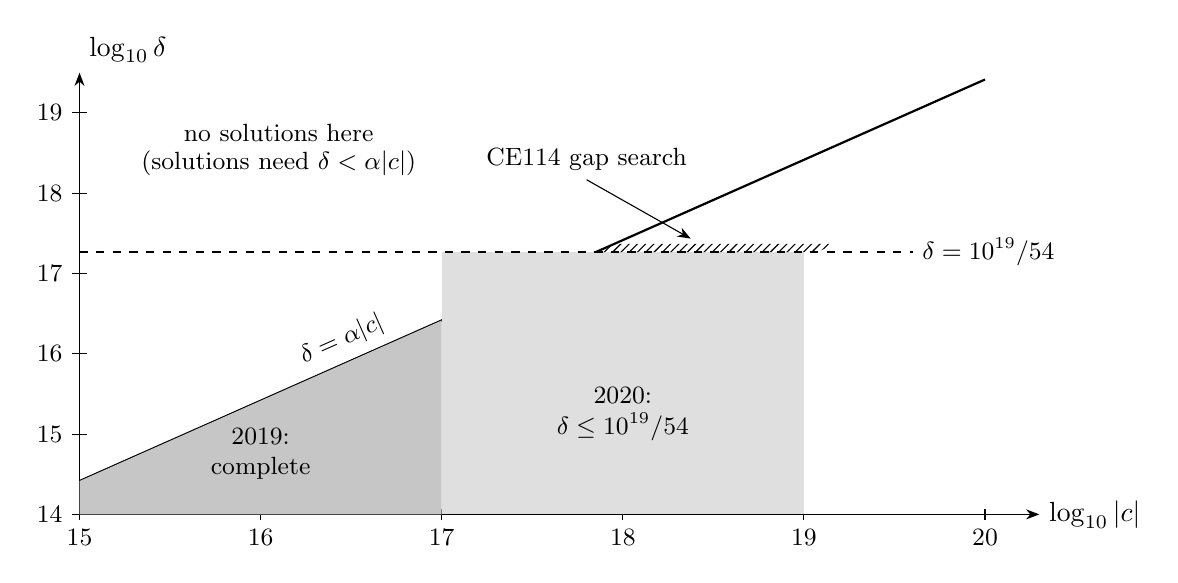
\begin{tikzpicture}[x=1.15cm,y=0.85cm]
  \draw[-{Stealth}] (0,0) -- (10.6,0) node[right] {$\log_{10}|c|$};
  \draw[-{Stealth}] (0,0) -- (0,6.6) node[above right] {$\log_{10}\delta$};
  % axis labels: x from 15 to 20, y from 14 to 19
  \foreach \v/\l in {0/15,2/16,4/17,6/18,8/19,10/20} \draw (\v,0.08)--(\v,-0.08) node[below]{\small $\l$};
  \foreach \v/\l in {0/14,1.2/15,2.4/16,3.6/17,4.8/18,6/19} \draw (0.08,\v)--(-0.08,\v) node[left]{\small $\l$};
  % delta < alpha|c| boundary: log delta = log c - 0.585 ; mapping x=2(logc-15), y=1.2(logd-14)
  \draw[thick] (0,{1.2*(15-0.585-14)}) -- (10,{1.2*(20-0.585-14)}) node[above,sloped,pos=0.3]{\small $\delta=\alpha|c|$};
  % 2019 complete: c<=1e17 (x<=4) below the boundary
  \fill[gray!45] (0,0) -- (4,0) -- (4,{1.2*(17-0.585-14)}) -- (0,{1.2*(15-0.585-14)}) -- cycle;
  % 2020: c<=1e19 (x<=8), delta <= 1.852e17 (y=1.2*(17.2676-14)=3.92)
  \fill[gray!25] (4,0) -- (8,0) -- (8,3.92) -- (4,3.92) -- cycle;
  \draw[dashed] (0,3.92) -- (9.2,3.92) node[right]{\small $\delta=10^{19}/54$};
  % gap region searched: delta from 1.852e17 slightly up, c in [3.847 delta, 64 delta]
  \fill[pattern=north east lines] ({2*(17.2676+0.585-15)},3.92) -- ({2*(17.2676+1.806-15)},3.92) -- ({2*(17.3676+1.806-15)},{1.2*(17.3676-14)}) -- ({2*(17.3676+0.585-15)},{1.2*(17.3676-14)}) -- cycle;
  \draw[-{Stealth}] (5.6,5.0) node[above]{\small CE114 gap search} -- (6.75,4.12);
  \node[align=center,font=\small] at (2.0,0.9) {2019:\\complete};
  \node[align=center,font=\small] at (6.0,1.5) {2020:\\$\delta\le10^{19}/54$};
  \node[font=\small] at (2.2,5.7) {no solutions here};
  \node[font=\small] at (2.2,5.25) {(solutions need $\delta<\alpha|c|$)};
\end{tikzpicture}
\caption{The $(|c|,\delta)$ plane for $k=114$, log scales. Shaded: searched by
Booker--Sutherland. Hatched: the strip searched by this campaign, just above
$\delta=10^{19}/54$, with $3.847\,\delta\le|c|\le64\,\delta$. The strip's height is
exaggerated: 1{,}800 core-hours cover a relative $\delta$-width of about $1.6\times10^{-4}$.}
\label{fig:plane}
\end{figure}

%====================================================================
\section{Rationale: where to spend 1,800 core-hours}\label{sec:rationale}

\subsection{Dr.\ Grechuk's critique of the earlier \texorpdfstring{$d$}{d}-first scripts}
The earlier 390 scripts enumerated rational slopes $d=p/q$ by height. A solution can be
reached only if $g=\gcd(A+B,A+C)$ is enormous, because its components have size about
$H(d)\cdot g$. The record solutions (for $k=33,42,3,165,579,906$) all have $g=1$, and the
largest value among them is $g=16$ (for $795$). Their heights are $H\sim10^{15}$--$10^{20}$.
For random pair sums $P(\gcd\ge G)\approx 6/(\pi^2G)$, so reaching beyond $10^{17}$ at
$H\le10^6$ has negligible probability. Dr.\ Grechuk's conclusion, to use the best known
method and aim it beyond the checked range, is adopted here.

\subsection{The density model}
Booker and Sutherland \cite[\S2.2]{BS} model the share of solutions with a given $\delta$ that
have $|c|/\delta\ge R$ as $cK(R)$, with $K(R)\sim R^{-1/2}$ and $c\approx1.96084$, so that
$cK(1/\alpha)=1$. Normalizing by Heath-Brown's conjectured count $e(B)=\rho\log B$ gives a
density in the $(\delta,|c|)$ plane of
\[
  dE=\frac{\rho}{2\sqrt\alpha}\,\delta^{-1/2}|c|^{-3/2}\,d\delta\,d|c|\qquad(\alpha|c|>\delta),
\]
with $\rho_{114}=0.058459$ from their Table~1. Two consequences follow.
\begin{enumerate}[leftmargin=*]
  \item Integrating over $|c|>\delta/\alpha$ gives $\rho/\delta$ expected solutions per
  $\delta$: solutions are \emph{log-uniform in $\delta$}.
  \item A band $|c|\le R\delta$ keeps a share $1-1/\sqrt{\alpha R}$, so
  \begin{equation}\label{eq:yield}
    E\bigl(\delta\in[D_0,D_1),\ |c|\le R\delta\bigr)=\rho\Bigl(1-\frac1{\sqrt{\alpha R}}\Bigr)\ln\frac{D_1}{D_0}.
  \end{equation}
\end{enumerate}

\subsection{Cost model and choice of region}
In the engine (Section~\ref{sec:engine}) most of the cost is fixed per $\delta$: sieving,
early rejection and cube roots. At $R=64$ the walk over $c$ adds only about $1.5$ candidates
per $\delta$. The figure that matters is therefore the \emph{yield per $\delta$},
$\rho(1-1/\sqrt{\alpha R})/\delta$. It is largest at the smallest unsearched $\delta$, which
is $D_0=10^{19}/54+1=185185185185185186$.

The alternatives are worse:
\begin{itemize}[leftmargin=*]
  \item Extending $|c|$ beyond $10^{19}$ for $\delta\le10^{19}/54$ means processing all
  $1.85\times10^{17}$ smaller $\delta$ again before any new $c$ is reached. That is millions
  of core-hours.
  \item Small pair sums with huge $|c|$, the direction of the folder's \code{xroots} and
  \code{xcurve}, hold almost nothing beyond $10^{19}$. Integrating the density over
  $\delta\le D$ and $|c|\ge10^{19}$ gives $2\rho\sqrt{D/(\alpha\cdot10^{19})}$, about
  $7\times10^{-9}$ for all $\delta\le10^4$ combined.
\end{itemize}

\subsection{Calibration and expected yield}
Calibration at $\delta\approx1.85\times10^{17}$ for $k=114$, with the 2-adic rule, on the
host of the 13 November revision (one core per measurement, \texttt{gap\_campaign.py
--calibrate}) gave:

\begin{center}
\begin{tabular}{rrrr}
\toprule
$R$ & $\mu$s per $\delta$ & coverage $1-1/\sqrt{\alpha R}$ & relative yield per core-second\\
\midrule
24 & 0.237 & 0.600 & $2.53\times10^6$\\
32 & 0.246 & 0.653 & $2.65\times10^6$\\
40 & 0.253 & 0.690 & $2.73\times10^6$\\
48 & 0.250 & 0.717 & $2.87\times10^6$\\
\textbf{64} & \textbf{0.265} & \textbf{0.755} & $\mathbf{2.85\times10^6}$\\
80 & 0.267 & 0.781 & $2.93\times10^6$\\
\bottomrule
\end{tabular}
\end{center}

The optimum is flat (within $3\%$ from $R=48$ to $80$) and $R=64$ is kept. With
$(R+18)\delta<2^{64}$ the hard ceiling is $R=81$ at this $\delta$.

The three versions of the engine were run back to back on the same host. Each ran twice on
each of two windows of $3\times10^7$ values of $\delta$ ($R=64$), and took, in $\mu$s per $\delta$:

\begin{center}
\begin{tabular}{lcc}
\toprule
engine & range & mean\\
\midrule
before the 2-adic rule & 0.314--0.326 & 0.319\\
with the 2-adic rule (Proposition~\ref{prop:twoadic}) & 0.247--0.252 & 0.250\\
with the 2-adic rule and the mod-24 wheel (current) & 0.240--0.246 & 0.243\\
\bottomrule
\end{tabular}
\end{center}

\noindent Together that is a factor of about $1.31$. The wheel's share is only about $3\%$:
the skipped $\delta$ were already cheap, since the sieve's division step returned at once for
them. The calibration table above was taken before the wheel. The original development host
measured $0.293\,\mu$s for the first engine, which corresponds to about $0.223\,\mu$s now. At that
speed, 1{,}800 core-hours cover $2.90\times10^{13}$ values of $\delta$, namely
$\delta\in[185185185185185186,\,185214218177221591)$. (It was $2.21\times10^{13}$ before.)
Equation~\eqref{eq:yield} then gives:

\begin{center}
\begin{tabularx}{\linewidth}{Yr}
\toprule
Use of 1,800 core-hours ($k=114$) & expected solutions\\
\midrule
This campaign, $0.223\,\mu$s per $\delta$ & $6.9\times10^{-6}$ (1 in 145{,}000)\\
This campaign, $0.243$--$0.255\,\mu$s (this revision's host) & 1 in 157{,}000--165{,}000\\
Before the 2-adic rule ($0.293\,\mu$s) & $5.3\times10^{-6}$ (1 in 190{,}000)\\
\code{xroots} (Algorithm D), 1,800 h inside its planned box & $\sim10^{-11}$\\
\code{xcurve} on every $|x|\le5000$, solved completely & $\sim7\times10^{-9}$ in total\\
\code{dsweep}, \code{dsmooth}, \code{xscan} & 0 (Section~\ref{sec:older})\\
\bottomrule
\end{tabularx}
\end{center}

\noindent The chance grows linearly with hours. Even so, this code can reach at most about
$0.9\%$ (about $2.5\times10^6$ core-hours at $0.223\,\mu$s per $\delta$) before $(R+18)\delta$ reaches $2^{64}$ at $R=64$.
These are heuristic figures, resting on Heath-Brown's conjecture and the Booker--Sutherland
model, not on theorems.

%====================================================================
\section{The engine: modus operandi}\label{sec:engine}

\begin{figure}[ht]
\centering
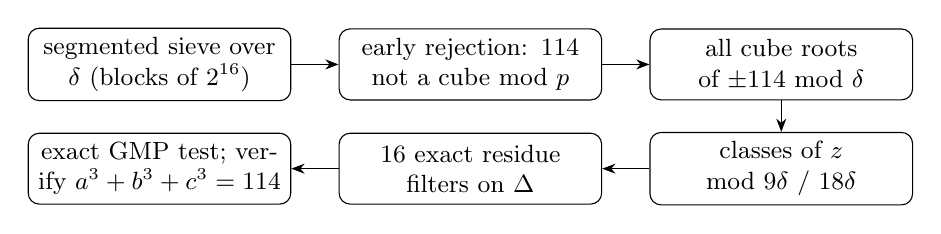
\begin{tikzpicture}[node distance=4mm and 6mm, box/.style={draw,rounded corners,align=center,font=\small,minimum height=9mm,text width=3.1cm}, >={Stealth}]
  \node[box] (s) {segmented sieve over $\delta$ (blocks of $2^{16}$)};
  \node[box,right=of s] (r) {early rejection: $114$ not a cube mod $p$};
  \node[box,right=of r] (c) {all cube roots of $\pm114$ mod $\delta$};
  \node[box,below=of c] (z) {classes of $z$ mod $9\delta$ / $18\delta$};
  \node[box,left=of z] (f) {16 exact residue filters on $\Delta$};
  \node[box,left=of f] (g) {exact GMP test; verify $a^3+b^3+c^3=114$};
  \draw[->] (s)--(r); \draw[->] (r)--(c); \draw[->] (c)--(z); \draw[->] (z)--(f); \draw[->] (f)--(g);
\end{tikzpicture}
\caption{Per-$\delta$ pipeline of \texttt{src/gap\_worker.cpp}. The mod-24 wheel keeps
$7/12$ of all $\delta$ out of the sieve ($3\mid\delta$, or excluded by the 2-adic rule). With
those that have no cube root, about $88\%$ of $\delta$ stop before the cube-root stage.}
\label{fig:pipe}
\end{figure}

The worker is \code{src/gap_worker.cpp} (C++17 with the GMP C API). It is invoked as
\texttt{gap\_worker --k 114 --d-start A --d-stop B --ratio-max 64} and processes every
$\delta\in[A,B)$. It is the engine written and reviewed for the 390 campaign, with $k=114$ as
its default.

\subsection{Sign and residue rules}
\begin{proposition}\label{prop:sign}
Let $k\equiv3\varepsilon\pmod9$, $\varepsilon=\pm1$; for $k=114$, $\varepsilon=-1$. Every
solution has $a\equiv b\equiv c\equiv\varepsilon\pmod3$. Hence $3\nmid\delta$,
$z\equiv\delta\pmod3$, and $\sgn(c)=+1$ exactly when $\delta\equiv\varepsilon\pmod3$. For 114,
$c>0$ exactly when $\delta\equiv2\pmod3$.
\end{proposition}
\begin{proof}
The first claim is the cube argument mod $9$. Then $a+b\equiv2\varepsilon\equiv-\varepsilon$,
so $3\nmid\delta$. For $|c|$ large, $(a-b)^2>0$ forces $\sgn(a+b)=-\sgn(c)$. If $c>0$ then
$a+b=-\delta\equiv-\varepsilon$, so $\delta\equiv\varepsilon$ and $z=c\equiv\varepsilon$. If
$c<0$ then $\delta=a+b\equiv-\varepsilon$ and $z=-c\equiv-\varepsilon$. In both cases
$z\equiv\delta\pmod 3$. This agrees with $s=\varepsilon(\delta/3)$ in \cite{BS}.
\end{proof}

\begin{proposition}[candidate test and converse]\label{prop:delta}
Put $K=k\,\sgn(c)$ and $\Delta=\bigl(4(z^3-K)/\delta-\delta^2\bigr)/3$. A pair $(\delta,z)$
with $z^3\equiv K\pmod\delta$ comes from a solution if and only if $\Delta=t^2$ for an integer
$t\equiv\delta\pmod2$. The solution is then $s_0=-\sgn(c)\delta$, $a=(s_0+t)/2$,
$b=(s_0-t)/2$, $c=\sgn(c)\,z$.
\end{proposition}
\begin{proof}
$a^3+b^3=s_0(s_0^2-3ab)=k-c^3$ gives $ab=(s_0^2-(k-c^3)/s_0)/3$. Then
$(a-b)^2=s_0^2-4ab=\Delta$. Conversely, such a $t$ makes $a,b$ integers with sum $s_0$ and
product $ab$, and $a^3+b^3+c^3=k$ follows. The worker re-checks this identity exactly.
\end{proof}

\begin{proposition}[classes of $z$]\label{prop:classes}
$9\mid\Delta$ for every solution, and $\Delta\bmod 9$ depends only on $z\bmod9\delta$. For
odd $\delta$, $\Delta\equiv1\pmod8$, and $\Delta\bmod8$ depends only on $z\bmod2$.
\end{proposition}
\begin{proof}
$a\equiv b\pmod3$ gives $9\mid(a-b)^2$. Write $3\delta\Delta=4(z^3-K)-\delta^3$. Replacing $z$
by $z+9\delta$ changes $z^3$ by a multiple of $27\delta$, so $3\delta\Delta\bmod27\delta$, and
hence $\Delta\bmod9$, depends only on $z\bmod9\delta$. For odd $\delta$, $t$ is odd, so
$\Delta=t^2\equiv1\pmod8$. Moreover $3\Delta\equiv4w-\delta^2\pmod8$ with
$w\equiv(z^3-K)\delta^{-1}\equiv z-K\pmod2$.
\end{proof}

\begin{proposition}[local conditions of Result~1]\label{prop:local}
Every point of Result~1 has $n\equiv0\pmod3$ and $x\equiv7\pmod{12}$. Every point of
Result~2 has $n\equiv0\pmod3$ and $X\equiv5$ or $11\pmod{12}$.
\end{proposition}
\begin{proof}
By Proposition~\ref{prop:charts}, $A,B,C\equiv2\pmod3$. Write each as $2+3u$; then
$(2+3u)^3\equiv8+9u\pmod{27}$, so $114\equiv24+9(u_A+u_B+u_C)\pmod{27}$, i.e.\
$u_A+u_B+u_C\equiv1\pmod3$. Hence $A+B+C=6+3\sum u\equiv0\pmod9$. It is also even, so
$18\mid A+B+C=6n$ and $3\mid n$. Next, $A+B\equiv1\pmod3$, so $x=-(A+B)/2\equiv1\pmod3$,
and in Result~2 $X=-(A+B)\equiv2\pmod3$ with $X$ odd. In Result~1, $A$ and $B$ are odd and
$C$ is even, so $C^3\equiv0\pmod8$. Odd $t$ satisfy $t^3\equiv t\pmod8$, so
$A+B\equiv A^3+B^3\equiv114\equiv2\pmod8$, and $x=-(A+B)/2\equiv3\pmod4$. Together these
give $x\equiv7\pmod{12}$.
\end{proof}

\noindent In Booker--Sutherland coordinates ($a+b=-\sgn(c)\,\delta$), $3\mid n$ reads
$z\equiv\delta\pmod9$. This is already enforced by the classes of
Proposition~\ref{prop:classes}: every one of the $154{,}376$ candidates walked on $10^5$
consecutive $\delta$ from $D_0$ satisfied it. The $2$-adic half of $x\equiv7\pmod{12}$, on
the other hand, was not used before. It is the following rule.

\begin{proposition}[2-adic rule for even $\delta$]\label{prop:twoadic}
Let $k\equiv2\pmod4$ (for example $k=114$) and let $\delta$ be even with
$\lfloor3.847\,\delta\rfloor^3>|k|$. Every solution with this $\delta$ in the walk satisfies
\[
  -\sgn(c)\,\delta\equiv k\pmod8 .
\]
For $k=114$, combined with Proposition~\ref{prop:sign}, the even $\delta$ that can occur are
$\delta\equiv10$ or $14\pmod{24}$: two of the eight even classes prime to $3$.
\end{proposition}
\begin{proof}
Since $k\equiv2\pmod4$, exactly one component is even (three even ones would give
$8\mid k$). If $\delta=|a+b|$ is even, $a,b$ have the same parity, so they are the odd pair
and $c$ is even. As in the previous proof, $a+b\equiv a^3+b^3=k-c^3\equiv k\pmod8$.
Moreover $a+b$ has the sign of $a^3+b^3=k-c^3$, and that sign is $-\sgn(c)$ when
$|c|^3>|k|$, which holds on the whole walk $|c|\ge\lfloor3.847\,\delta\rfloor$. So
$a+b=-\sgn(c)\,\delta$. For $114$: if $c>0$ then $\delta\equiv2\pmod3$ and
$-\delta\equiv2\pmod8$, so $\delta\equiv14\pmod{24}$. If $c<0$ then $\delta\equiv1\pmod3$
and $\delta\equiv2\pmod8$, so $\delta\equiv10\pmod{24}$.
\end{proof}

\noindent For $k=114$ this is exactly $x\equiv3\pmod4$ for the Result-1 point whose $C$ is
the smallest component. The worker never sieves the excluded $\delta$ (the wheel in
Section~\ref{sec:engine}), so it neither factors them nor looks for cube roots. It counts them as
\texttt{d\_skipped\_2adic}. \texttt{--no-filter} switches the rule off, for validation.

\subsection{Steps for each \texorpdfstring{$\delta$}{delta}}
\begin{enumerate}[leftmargin=*]
\item \textbf{Factor.} Primes up to $\sqrt{\delta_{\rm stop}}\approx4.3\times10^8$ are
generated once per task in about 1--3\,s. Primes below $2^{16}$ are applied directly to each
block of $2^{16}$ consecutive $\delta$. Larger primes live in buckets: linked lists of
fixed-size pages drawn from a shared free pool, each prime filed under the block of its next
multiple. The cofactor left after sieving is $1$ or a prime.

\emph{Wheel.} Only $\delta$ in the $10$ allowed classes mod $24$ are sieved: $1,5,7,11,13,
17,19,23$ and the even classes $10,14$ of Proposition~\ref{prop:twoadic}. Without the 2-adic
rule ($R<27$, \texttt{--no-filter}, or $k\not\equiv2\bmod4$) there are $16$ classes, and
\texttt{--dump-factors} uses all $24$. A prime $p\ge5$ is prime to $24$, so its multiple $mp$
lies in class $(m\bmod24)(p\bmod24)$, and the multipliers to visit are fixed classes of $m$.
A table gives the step from each allowed $m$ to the next. Each bucket entry carries
$m\bmod24$ in spare bits, and the bucket ring is widened by the largest step ($4$). The
primes $2$ and $3$ are stepped as before. Over $4\times10^9$ values of $\delta$ from $D_0$
(about $2.3$ bucket cycles) the peak memory was $0.232$\,GB, at a sustained
$0.246\,\mu$s per $\delta$ and $3.6$\,s of set-up.
\item \textbf{Reject early.} A prime $p\equiv1\pmod3$ dividing $\delta$ for which $114$ is
not a cube mod $p$ leaves no root. This is precomputed per prime, packed into the bucket
entries, and applied before any division. Similarly $p\mid114$ with $v_p(114)=1$ and
$p^2\mid\delta$ leaves no root. One third of all $\delta$ are skipped because $3\mid\delta$,
and a quarter by the 2-adic rule (Proposition~\ref{prop:twoadic}). Of the rest, about
$29\%$ of all $\delta$ have no root, so only about $12\%$ remain.
\item \textbf{Cube roots of $K$ mod $\delta$.}
  \begin{itemize}
    \item $p\equiv2\pmod3$: $K^{(2p-1)/3}$.
    \item $p\equiv1\pmod3$: Adleman--Manders--Miller in the $3$-Sylow subgroup, with a
    single-exponentiation fast path when $p\equiv4,7\pmod9$.
    \item Then Hensel lifting to $p^e$, brute force for $p\mid114$, and CRT across the
    factors.
  \end{itemize}
  Roots of $-114$ are the negatives of roots of $114$. Exponentiations use 64-bit
  Montgomery arithmetic.
\item \textbf{Walk.} For each root, keep the classes modulo $9\delta$ (or $18\delta$ for odd
$\delta$) allowed by Propositions~\ref{prop:sign} and~\ref{prop:classes}. Walk them over
$\lfloor3847\delta/1000\rfloor\le z\le R\delta$. Since $3.847<1/\alpha=3.84732\ldots$, no
admissible $z$ is skipped; the $k$-correction to Lemma~\ref{lem:bs} is about $10^{-30}$
relative.
\item \textbf{Filter.} For each of the $16$ primes $5\le p\le61$ not dividing $\delta$, test
that $\Delta\equiv A_pz^3+B_p\pmod p$ is a square (zero included), with $A_p=4/(3\delta)$ and
$B_p=-4K/(3\delta)-\delta^2/3$. Each test is a necessary condition, compiled with a constant
modulus.
\item \textbf{Decide and verify.} For survivors, compute $\Delta$ exactly with GMP, test
whether it is a perfect square with $t\equiv\delta\pmod2$, rebuild $(a,b,c)$ by
Proposition~\ref{prop:delta}, and verify $a^3+b^3+c^3=114$. The hit is printed as a JSON
line.
\end{enumerate}

Measured on 16 million $\delta$ starting at $D_0$ ($k=114$, $R=64$, with the 2-adic
rule):

\begin{center}
\begin{tabular}{lrr}
\toprule
counter & total & per $\delta$\\
\midrule
$\delta$ skipped, $3\mid\delta$ & 5{,}333{,}333 & 0.333\\
$\delta$ skipped by the 2-adic rule & 3{,}999{,}999 & 0.250\\
$\delta$ with no cube root & 4{,}679{,}745 & 0.292\\
$\delta$ processed further & 1{,}986{,}923 & 0.124\\
cube roots & 4{,}618{,}747 & 0.289\\
candidates $z$ & 18{,}524{,}758 & 1.16\\
passed the residue filters (exact GMP checks) & 647 & $4.0\times10^{-5}$\\
solutions & 0 & --\\
\bottomrule
\end{tabular}
\end{center}

\paragraph{Overflow guards.} The worker refuses to start unless $27\delta_{\rm stop}<2^{63}$
and $(R+18)\delta_{\rm stop}<2^{64}$. The 2-adic residue of $\Delta$ is computed exactly mod
$2^{64}$ using $\delta^{-1}$ and $3^{-1}$. All other modular products stay within 128 bits.

%====================================================================
\section{From a solution to the rational \texorpdfstring{$d$}{d}: \texttt{to\_d.py}}

\code{to_d.py} reads \code{hits.jsonl} (or raw worker output, skipping non-hit records), or a
single triple via \texttt{--triple A B C}. It removes duplicate representations and, for each
choice of $C$, applies Proposition~\ref{prop:charts}. Before printing, it checks every point
with exact rationals:
\begin{itemize}
  \item $s\ge0$ and $s^2=(x+6n)^2+N/x$;
  \item equation \eqref{eq:E} holds with this $d$;
  \item the chart: $x,s\in\mathbb Z$ (Result~1), or both with denominator $2$, so that
  $X=2x$ and $Y=2s$ are odd (Result~2).
\end{itemize}
Output, one line per point:
\begin{center}
\texttt{result 2 (half chart): d = ... n = ... x = .../2 sqrt = .../2 X=... Y=...}
\end{center}
By Proposition~\ref{prop:three}, a representation of $114$ always produces exactly one
Result-1 line and two Result-2 lines.

%====================================================================
\section{Operating the 1,800-core-hour campaign}
\begingroup\sloppy

\begin{enumerate}[leftmargin=*]
\item \textbf{Build and test:} \texttt{make \&\& make test} (20 tests, about 150\,s). Or
\texttt{docker build .}, which compiles the worker and runs the test suite during the build.
\item \textbf{Calibrate} on Charity Engine's CPU type: \texttt{python3 gap\_campaign.py
--calibrate}. It prints the $\mu$s per $\delta$ for several $R$ and the best $R$.
\item \textbf{Plan:} \texttt{python3 gap\_campaign.py --campaign-id ce114-gap}
\texttt{--ratio-max 64} \texttt{--us-per-d <measured>} \texttt{--output-dir gap-tasks}. The defaults are $k=114$, 1{,}800 core-hours
and $D_0=185185185185185186$. The range is split evenly into tasks of about one hour each
(1{,}800 tasks; always pass the $\mu$s per $\delta$ measured on the grid), and \code{page.json} is written with the heuristic yield.
Nothing is submitted.
\item \textbf{Run} each task: \texttt{python3 run\_gap\_task.py --task <task.json>
--output-dir <dir>}. In the container this is the default command, on
\code{/local/input/task.json}.
  \begin{itemize}
    \item The runner verifies each hit exactly before storing it.
    \item It writes an fsynced checkpoint every $2^{24}$ values of $\delta$, recording the
    exact interval $[\text{covered\_start},\text{d\_next})$ this directory has searched.
    \item It resumes in place. It refuses to resume if the task would start before that
    interval, so no unsearched range is ever credited.
    \item On SIGTERM it stops the worker and writes \code{continuation.task.json}.
    \item Exit code: 0 for complete or partial; \texttt{--partial-exit-code} can make
    partial runs non-zero so the grid retries them.
  \end{itemize}
\item \textbf{Collect:} \texttt{collect\_gap.py --page ... --results ... --output-dir ...}
unions the checkpoint intervals and validates them against tasks and page. It reports gaps
(exit 2 with \texttt{--require-complete}), re-verifies every hit, and sums worker core-hours.
\item \textbf{Audit:} \texttt{audit\_gap.py --fraction 0.02} re-runs a random 2\% of returned
chunks on trusted hardware and compares their deterministic counters. Any mismatch flags a
faulty host; that task is re-issued.
\item \textbf{Convert:} \texttt{python3 to\_d.py gap-collected/hits.jsonl}.
\end{enumerate}

\endgroup
\noindent\textbf{Resources.} About $0.23$--$0.24$\,GB of memory, 1--4\,s of set-up per task,
single-threaded. Set-up and the 2\% audit (about 36 core-hours) come on top of the 1{,}800
hours and should be kept within the project's headroom.

%====================================================================
\section{Validation and review}

\subsection{Tests (\texttt{make test})}
\begin{itemize}[leftmargin=*]
\item \textbf{Record solutions.} From $\pm25$-wide $\delta$ windows the worker rediscovers the
known solutions for $k=33,42,3,165,579,795,906$. These include 579, found in the same 2020
run that covered 114, and $k=3$ at $|c|/\delta\approx4.4\times10^6$. Excluding the window
loses the hit, and disabling every filter changes nothing.
\item \textbf{Brute force.} For every $k\equiv\pm3\pmod9$ up to 100, the worker finds all
solutions with coordinates up to $2000$ in the searched region, and nothing else.
\item \textbf{2-adic rule.} The current engine and the engine before the rule return
identical hits for all $55$ values $k<1000$ with $k\equiv2\pmod4$ and $k\equiv\pm3\pmod9$,
over $1\le\delta<3\times10^6$ with $|c|\le1000\,\delta$ ($143$ representations). The test
suite repeats this against \texttt{--no-filter} for $k=6,42,222,438,618$. It also checks the
congruence on every even-$\delta$ hit, and that the skip was active.
\item \textbf{Wheel.} On two windows of $2\times10^6$ values of $\delta$ (from $D_0$ and from
$1000003$), every deterministic counter equals that of the engine before the wheel: the same
$\delta$ are skipped and have roots, with the same roots, candidates and exact checks. On
$16\times10^6$ $\delta$ from $D_0$ the counters also agree. This is a test in the suite.
\item \textbf{Filter decisions.} On production-size candidates for $k=114,390,627,33$, every
2-adic and residue decision agrees with exact integer arithmetic.
\item \textbf{Factorizations and roots.} Factorizations near $D_0$ and near $2^{58}$ are
checked by product and primality. Root sets are checked by brute force for $\delta<1500$,
and by multiplicativity at production size for $k=114$ and $390$, including $\delta$
divisible by $2^{25}$, $5^{14}$, $7^{12}$ and $13^{10}$.
\item \textbf{Converter.}
  \begin{itemize}
    \item The $42$ and $906$ records give $1+2$ points satisfying \eqref{eq:E}, with the same
    $d$ as the folder's independent \code{grid/verify.py}.
    \item A brute force over \eqref{eq:E} itself ($|n|\le25$, $0<|X|\le120$, nine values of
    $m$ including $19$) confirms that every acceptable point is a representation and is
    listed. For $m=19$ there are none, as Booker--Sutherland's bound implies.
    \item Raw worker output and duplicated hits are handled; a repeated component gives two
    points.
  \end{itemize}
\item \textbf{Lifecycle.} Plan, run, SIGTERM, resume and collect work end to end. Re-running
an original task where its continuation ran is refused, a same-directory continuation leaves
no false gap, and the audit detects a counter altered by one.
\end{itemize}

\subsection{Pilot}
A pilot over $\delta\in[D_0,D_0+2\times10^9)$ ($R=64$) ran through the full pipeline. It used
0.173 core-hours (0.31\,$\mu$s per $\delta$ on a shared host), returned no solutions, left
no gaps, and 6 of 6 audited chunks agreed. The record is in \code{gap-search/validation/pilot/}.

\subsection{Independent reviews}
Two separate reviews read the code without being given the author's conclusions.
\begin{itemize}[leftmargin=*]
  \item \textbf{The engine.} The first review re-checked roots, factorizations, the $z$-walk
  and filter decisions on several million further $\delta$ and $10^5$ further candidates,
  and found no way to miss a solution. Its findings on coverage accounting, durability, the
  mod-$9\delta$ speed-up and the figures were all adopted.
  \item \textbf{The 114 parts.} The second review covered the converter, the equivalence
  claims, the 114 port and the documentation. It confirmed the identity, the congruences, the
  yield arithmetic and the search boundary. Its corrections (the description of the older
  engines, distinctness of components, reach of the code, CLI details, even task split) were
  applied in commit \texttt{194e6ca}.
\end{itemize}

%====================================================================
\section{Status of the folder's earlier programs}\label{sec:older}

The earlier programs in \code{grid/} and \code{search/} remain for reproducibility. In the
light of Section~\ref{sec:excluded} they are not the place where an acceptable result can
come from:

\begin{center}
\begin{tabularx}{\linewidth}{lY}
\toprule
program & status for Results 1 and 2\\
\midrule
\code{dsweep}, \code{dsmooth} & They enumerate the certificate $U=2dx^2$ (or $V=dX^2$) and do
have integral modes. But an acceptable point needs $|V|\ge5.8\cdot10^{24}$; \code{dsweep}
stops at $10^{18}$, and \code{dsmooth} reaches that size only for $B$-smooth certificates.\\
\code{xscan} & Scans $n$-windows far below the required $|n|\ge9.8\cdot10^{15}$.\\
\code{xcurve} & Unbounded in $n$ for each fixed $x$, but small $|x|$ (small pair sums)
holds about $7\times10^{-9}$ expected solutions beyond $|c|=10^{19}$ for all $|x|\le5000$.\\
\code{xroots} (Algorithm D) & Correct and complete for its boxes, but aimed at small
$|X|<10^6$ with $|n|$ beyond $10^{18}$: about $10^{-11}$ per 1{,}800 hours.\\
\code{rational-d-search/} (new) & Every $(n,x)$ in both charts whose square root is merely
\emph{rational}, complete in $x$ for each $n$. It factors $36n^3-19$ completely (rho and
ECM), matches a brute force for $|n|\le450$, and re-finds the eleven known integer-chart
points. It is a cross-check only: its points are not Results~1 or~2.\\
\code{RequestProject/*.lean} & Lean proofs of the reduction, the small-$|n|$ completeness
and the earlier algorithms; unaffected.\\
\bottomrule
\end{tabularx}
\end{center}

\noindent The rational-$d$ points with non-integral radicals found by those programs (for
example $d=-142/4913$ at $(n,x)=(15,-289/2)$, or the new $d=-41449/33275$ at
$(309,15125/2)$ from \code{rational-d-search}) are genuine points of \eqref{eq:E}. They are
not Results~1 or 2.

%====================================================================
\section{What a run proves, and its limits}

A completed and audited campaign proves that \eqref{eq:E} has \emph{no} point of Result~1
or~2 arising from a representation with $\delta=|a+b|$ in the covered range and
$3.847\,\delta\le|c|\le64\,\delta$. Equivalently, it proves that $114$ has no representation
in that region. This is a new, exact exclusion region that does not depend on any heuristic.

It does not cover other $\delta$, or $|c|$ outside the band. The probability figures of
Section~\ref{sec:rationale} are heuristic. Three things would raise the odds:
\begin{itemize}
  \item more core-hours, since the gain is linear;
  \item Booker and Sutherland's own implementation, which a rough comparison with their
  $k=33$ benchmark suggests may be about three times faster per $\delta$;
  \item confirming with them, or with Charity Engine, that the region has not been searched
  since 2020.
\end{itemize}

%====================================================================
\appendix
\section{Files}
\begin{center}
\begin{tabularx}{\linewidth}{lY}
\toprule
file (in \code{gap-search/}) & role\\
\midrule
\code{src/gap_worker.cpp} & the engine (Section~\ref{sec:engine})\\
\code{gap_common.py} & shared validation, exact hit verification, density table, yield formula\\
\code{gap_campaign.py} & calibration, budget sizing, task and \code{page.json} generation\\
\code{run_gap_task.py} & restartable task runner with checkpoints and continuation\\
\code{collect_gap.py} & coverage union, gap report, hit re-verification\\
\code{audit_gap.py} & re-runs sampled chunks to detect faulty hosts\\
\code{to_d.py} & representation $\to$ the three rational $d$, verified on \eqref{eq:E}\\
\code{tests/} & \code{test_gap.py} (engine, 14 tests), \code{test_to_d.py} (converter, 6 tests)\\
\code{Dockerfile}, \code{container_entrypoint.sh} & Charity Engine image (tests run at build)\\
\code{examples/pilot/}, \code{validation/pilot/} & pilot tasks and its collected summary\\
\code{README.md} & short operating guide\\
\bottomrule
\end{tabularx}
\end{center}

\begin{thebibliography}{9}
\bibitem{BS} A.~R. Booker and A.~V. Sutherland, \emph{On a question of Mordell},
Proc.\ Natl.\ Acad.\ Sci.\ USA \textbf{118} (2021), e2022377118; arXiv:2007.01209.
\bibitem{HB} D.~R. Heath-Brown, \emph{The density of zeros of forms for which weak approximation
fails}, Math.\ Comp.\ \textbf{59} (1992), 613--623.
\end{thebibliography}

\end{document}
